%% LyX 1.3 created this file.  For more info, see http://www.lyx.org/.
%% Do not edit unless you really know what you are doing.
\documentclass[english]{article}
\usepackage{bookman}
\usepackage[T1]{fontenc}
\usepackage[latin1]{inputenc}
\usepackage{geometry}
\geometry{verbose,a4paper,tmargin=20mm,bmargin=20mm}
\usepackage{graphicx}
\IfFileExists{url.sty}{\usepackage{url}}
                      {\newcommand{\url}{\texttt}}

\makeatletter

%%%%%%%%%%%%%%%%%%%%%%%%%%%%%% LyX specific LaTeX commands.
%% Bold symbol macro for standard LaTeX users
\newcommand{\boldsymbol}[1]{\mbox{\boldmath $#1$}}

%% Because html converters don't know tabularnewline
\providecommand{\tabularnewline}{\\}

%%%%%%%%%%%%%%%%%%%%%%%%%%%%%% Textclass specific LaTeX commands.
 \newenvironment{lyxcode}
   {\begin{list}{}{
     \setlength{\rightmargin}{\leftmargin}
     \setlength{\listparindent}{0pt}% needed for AMS classes
     \raggedright
     \setlength{\itemsep}{0pt}
     \setlength{\parsep}{0pt}
     \normalfont\ttfamily}%
    \item[]}
   {\end{list}}

%%%%%%%%%%%%%%%%%%%%%%%%%%%%%% User specified LaTeX commands.
% header
\usepackage{fancyhdr}
\pagestyle{fancy}
\lhead{Structural Biopython FAQ}
\rhead{}

% remove date
\date{}

% make everything have section numbers
% Make links between references
\usepackage{hyperref}

\newif\ifpdf
\ifx\pdfoutput\undefined
  \pdffalse
\else
  \pdfoutput=1
  \pdftrue
\fi
\ifpdf
  \hypersetup{colorlinks=true, hyperindex=true, citecolor=red, urlcolor=blue}
\fi

\usepackage{babel}
\makeatother
\begin{document}

\title{{\huge The Biopython}\\
{\huge Structural Bioinformatics FAQ}}


\author{Thomas Hamelryck}


\author{{\normalsize Bioinformatics center}\\
{\normalsize Institute of Molecular Biology}\\
{\normalsize University of Copenhagen }\\
{\normalsize Universitetsparken 15, Bygning 10}\\
{\normalsize DK-2100 K�benhavn �}\\
{\normalsize Denmark }\\
{\normalsize thamelry@binf.ku.dk}\\
\url{http://www.binf.ku.dk/users/thamelry/}}

\maketitle

\section{Introduction}

The Biopython Project is an international association of developers
of freely available Python (\url{http://www.python.org}) tools for
computational molecular biology. Python is an object oriented, interpreted,
flexible language that is becoming increasingly popular for scientific
computing. Python is easy to learn, has a very clear syntax and can
easily be extended with modules written in C, C++ or FORTRAN.

The Biopython web site (\url{http://www.biopython.org}) provides
an online resource for modules, scripts, and web links for developers
of Python-based software for bioinformatics use and research. Basically,
the goal of biopython is to make it as easy as possible to use python
for bioinformatics by creating high-quality, reusable modules and
classes. Biopython features include parsers for various Bioinformatics
file formats (BLAST, Clustalw, FASTA, Genbank,...), access to online
services (NCBI, Expasy,...), interfaces to common and not-so-common
programs (Clustalw, DSSP, MSMS...), a standard sequence class, various
clustering modules, a KD tree data structure etc. and even documentation. 

Bio.PDB is a biopython module that focuses on working with crystal
structures of biological macromolecules. This document gives a fairly
complete overview of Bio.PDB.


\section{Bio.PDB's installation}

Bio.PDB is automatically installed as part of Biopython. Biopython
can be obtained from \url{http://www.biopython.org}. It runs on many
platforms (Linux/Unix, windows, Mac,...).

However, the \verb|Bio.PDB.mmCIF.MMCIFlex| module (used internally by
\verb|Bio.PDB.MMCIFParser| to parse mmCIF files) is \emph{not} currently
installed by default.  This module relies on a third party tool called
flex (fast lexical analyzer generator).
At the time of writing, in order to parse mmCIF files you'll have to
install flex, then tweak your \verb|setup.py| file and (re)install
Biopython from source.

\section{Who's using Bio.PDB?}

Bio.PDB was used in the construction of DISEMBL, a web server that
predicts disordered regions in proteins (\url{http://dis.embl.de/}),
and COLUMBA, a website that provides annotated protein structures
(\url{http://www.columba-db.de/}). Bio.PDB has also been used to
perform a large scale search for active sites similarities between
protein structures in the PDB (see \textit{Proteins Struct. Func.
Gen.}, \textbf{2003}, 51, 96-108), and to develop a new algorithm
that identifies linear secondary structure elements (\emph{BMC Bioinformatics},
\textbf{2005}, 6, 202, \url{http://www.biomedcentral.com/1471-2105/6/202}). 

Judging from requests for features and information, Bio.PDB is also
used by several LPCs (Large Pharmaceutical Companies :-).


\section{Is there a Bio.PDB reference?}

Yes, and I'd appreciate it if you would refer to Bio.PDB in publications
if you make use of it. The reference is:

\begin{quote}
Hamelryck, T., Manderick, B. (2003) PDB parser and structure class
implemented in Python. \textit{Bioinformatics}, \textbf{19}, 2308-2310. 
\end{quote}
The article can be freely downloaded via the Bioinformatics journal
website (\url{http://www.binf.ku.dk/users/thamelry/references.html}).
I welcome e-mails telling me what you are using Bio.PDB for. Feature
requests are welcome too.


\section{How well tested is Bio.PDB?}

Pretty well, actually. Bio.PDB has been extensively tested on nearly
5500 structures from the PDB - all structures seemed to be parsed
correctly. More details can be found in the Bio.PDB Bioinformatics
article. Bio.PDB has been used/is being used in many research projects
as a reliable tool. In fact, I'm using Bio.PDB almost daily for research
purposes and continue working on improving it and adding new features.


\section{How fast is it?}

The \texttt{PDBParser} performance was tested on about 800 structures
(each belonging to a unique SCOP superfamily). This takes about 20
minutes, or on average 1.5 seconds per structure. Parsing the structure
of the large ribosomal subunit (1FKK), which contains about 64000
atoms, takes 10 seconds on a 1000 MHz PC. In short: it's more than
fast enough for many applications.


\section{Why should I use Bio.PDB?}

Bio.PDB might be exactly what you want, and then again it might not.
If you are interested in data mining the PDB header, you might want
to look elsewhere because there is only limited support for this.
If you look for a powerful, complete data structure to access the
atomic data Bio.PDB is probably for you. 


\section{Usage}


\subsection{General questions}


\subsubsection*{Importing Bio.PDB}

That's simple:

\begin{lyxcode}
from~Bio.PDB~import~{*}
\end{lyxcode}

\subsubsection*{Is there support for molecular graphics?}

Not directly, mostly since there are quite a few Python based/Python
aware solutions already, that can potentially be used with Bio.PDB.
My choice is Pymol, BTW (I've used this successfully with Bio.PDB,
and there will probably be specific PyMol modules in Bio.PDB soon/some
day). Python based/aware molecular graphics solutions include:

\begin{itemize}
\item PyMol: \url{http://pymol.sourceforge.net/}
\item Chimera: \url{http://www.cgl.ucsf.edu/chimera/}
\item PMV: \url{http://www.scripps.edu/~sanner/python/}
\item Coot: \url{http://www.ysbl.york.ac.uk/~emsley/coot/}
\item CCP4mg: \url{http://www.ysbl.york.ac.uk/~lizp/molgraphics.html}
\item mmLib: \url{http://pymmlib.sourceforge.net/} 
\item VMD: \url{http://www.ks.uiuc.edu/Research/vmd/}
\item MMTK: \url{http://starship.python.net/crew/hinsen/MMTK/}
\end{itemize}
I'd be crazy to write another molecular graphics application (been
there - done that, actually :-).


\subsection{Input/output}


\subsubsection*{How do I create a structure object from a PDB file?}

First, create a \texttt{PDBParser} object:

\begin{lyxcode}
parser=PDBParser()
\end{lyxcode}
Then, create a structure object from a PDB file in the following way
(the PDB file in this case is called '1FAT.pdb', 'PHA-L' is a user
defined name for the structure):

\begin{lyxcode}
structure=parser.get\_structure('PHA-L',~'1FAT.pdb')
\end{lyxcode}

\subsubsection*{How do I create a structure object from an mmCIF file?}

Similarly to the case the case of PDB files, first create an \texttt{MMCIFParser}
object:

\begin{lyxcode}
parser=MMCIFParser()
\end{lyxcode}
Then use this parser to create a structure object from the mmCIF file:

\begin{lyxcode}
structure=parser.get\_structure('PHA-L',~'1FAT.cif')
\end{lyxcode}

\subsubsection*{...and what about the new PDB XML format?}

That's not yet supported, but I'm definitely planning to support that
in the future (it's not a lot of work). Contact me if you need this,
it might encourage me :-).


\subsubsection*{I'd like to have some more low level access to an mmCIF file...}

You got it. You can create a python dictionary that maps all mmCIF
tags in an mmCIF file to their values. If there are multiple values
(like in the case of tag \texttt{\_atom\_site.Cartn\_y}, which holds
the y coordinates of all atoms), the tag is mapped to a list of values.
The dictionary is created from the mmCIF file as follows:

\begin{lyxcode}
mmcif\_dict=MMCIF2Dict('1FAT.cif')
\end{lyxcode}
Example: get the solvent content from an mmCIF file:

\begin{lyxcode}
sc=mmcif\_dict{[}'\_exptl\_crystal.density\_percent\_sol'{]}
\end{lyxcode}
Example: get the list of the y coordinates of all atoms

\begin{lyxcode}
y\_list=mmcif\_dict{[}'\_atom\_site.Cartn\_y'{]}
\end{lyxcode}

\subsubsection*{Can I access the header information?}

Thanks to Christian Rother you can access some information from the
PDB header. Note however that many PDB files contain headers with
incomplete or erroneous information. Many of the errors have been
fixed in the equivalent mmCIF files. \emph{Hence, if you are interested
in the header information, it is a good idea to extract information
from mmCIF files using the} \texttt{\emph{MMCIF2Dict}} \emph{tool
described above, instead of parsing the PDB header. }

Now that is clarified, let's return to parsing the PDB header. The
structure object has an attribute called \texttt{header} which is
a python dictionary that maps header records to their values.

Example:

\begin{lyxcode}
resolution=structure.header{[}'resolution'{]}

keywords=structure.header{[}'keywords'{]}
\end{lyxcode}
The available keys are \texttt{name, head, deposition\_\-date, release\_\-date,
structure\_\-method, resolution, structure\_\-reference} (maps to
a list of references), \texttt{journal\_\-reference, author} and
\texttt{compound} (maps to a dictionary with various information about
the crystallized compound).

The dictionary can also be created without creating a \texttt{Structure}
object, ie. directly from the PDB file:

\begin{lyxcode}
file=open(filename,'r')

header\_dict=parse\_pdb\_header(file)

file.close()
\end{lyxcode}

\subsubsection*{Can I use Bio.PDB with NMR structures (ie. with more than one model)?}

Sure. Many PDB parsers assume that there is only one model, making
them all but useless for NMR structures. The design of the \texttt{Structure}
object makes it easy to handle PDB files with more than one model
(see section \ref{sub:The-Structure-object}). 


\subsubsection*{How do I download structures from the PDB?}

This can be done using the \texttt{PDBList} object, using the \texttt{retrieve\_pdb\_file}
method. The argument for this method is the PDB identifier of the
structure.

\begin{lyxcode}
pdbl=PDBList()

pdbl.retrieve\_pdb\_file('1FAT')
\end{lyxcode}
The \texttt{PDBList} class can also be used as a command-line tool: 

\begin{lyxcode}
python~PDBList.py~1fat
\end{lyxcode}
The downloaded file will be called \texttt{pdb1fat.ent} and stored
in the current working directory. Note that the \texttt{retrieve\_pdb\_file}
method also has an optional argument \texttt{pdir} that specifies
a specific directory in which to store the downloaded PDB files. 

The \texttt{retrieve\_pdb\_file} method also has some options to specify
the compression format used for the download, and the program used
for local decompression (default \texttt{.Z} format and \texttt{gunzip}).
In addition, the PDB ftp site can be specified upon creation of the
\texttt{PDBList} object. By default, the RCSB PDB server (\url{ftp://ftp.rcsb.org/pub/pdb/data/structures/divided/pdb/})
is used. See the API documentation for more details. Thanks again
to Kristian Rother for donating this module.


\subsubsection*{How do I download the entire PDB?}

The following commands will store all PDB files in the \texttt{/data/pdb}
directory: 

\begin{lyxcode}
python~PDBList.py~all~/data/pdb~

python~PDBList.py~all~/data/pdb~-d~
\end{lyxcode}
\noindent The API method for this is called \texttt{download\_entire\_pdb}.
Adding the \texttt{-d} option will store all files in the same directory.
Otherwise, they are sorted into PDB-style subdirectories according
to their PDB ID's. Depending on the traffic, a complete download will
take 2-4 days. 


\subsubsection*{How do I keep a local copy of the PDB up-to-date?}

This can also be done using the \texttt{PDBList} object. One simply
creates a \texttt{PDBList} object (specifying the directory where
the local copy of the PDB is present) and calls the \texttt{update\_pdb}
method:

\begin{lyxcode}
pl=PDBList(pdb='/data/pdb')

pl.update\_pdb()
\end{lyxcode}
One can of course make a weekly \texttt{cronjob} out of this to keep
the local copy automatically up-to-date. The PDB ftp site can also
be specified (see API documentation).

\texttt{PDBList} has some additional methods that can be of use. The
\texttt{get\_all\_obsolete} method can be used to get a list of all
obsolete PDB entries. The \texttt{changed\_this\_week} method can
be used to obtain the entries that were added, modified or obsoleted
during the current week. For more info on the possibilities of \texttt{PDBList},
see the API documentation.


\subsubsection*{What about all those buggy PDB files?}

It is well known that many PDB files contain semantic errors (I'm
not talking about the structures themselves know, but their representation
in PDB files). Bio.PDB tries to handle this in two ways. The PDBParser
object can behave in two ways: a restrictive way and a permissive
way (THIS IS NOW THE DEFAULT). The restrictive way used to be the
default, but people seemed to think that Bio.PDB 'crashed' due to
a bug (hah!), so I changed it. If you ever encounter a real bug, please
tell me immediately!

Example:

\begin{lyxcode}
\#~Permissive~parser

parser=PDBParser(PERMISSIVE=1)

parser=PDBParser()~\#~The~same~(default)

\#~Strict~parser

strict\_parser=PDBParser(PERMISSIVE=0)
\end{lyxcode}
In the permissive state (DEFAULT), PDB files that obviously contain
errors are 'corrected' (ie. some residues or atoms are left out).
These errors include:

\begin{itemize}
\item Multiple residues with the same identifier
\item Multiple atoms with the same identifier (taking into account the altloc
identifier)
\end{itemize}
These errors indicate real problems in the PDB file (for details see
the Bioinformatics article). In the restrictive state, PDB files with
errors cause an exception to occur. This is useful to find errors
in PDB files.

Some errors however are automatically corrected. Normally each disordered
atom should have a non-blanc altloc identifier. However, there are
many structures that do not follow this convention, and have a blank
and a non-blank identifier for two disordered positions of the same
atom. This is automatically interpreted in the right way.

Sometimes a structure contains a list of residues belonging to chain
A, followed by residues belonging to chain B, and again followed by
residues belonging to chain A, i.e. the chains are 'broken'. This
is also correctly interpreted.


\subsubsection*{Can I write PDB files?}

Use the PDBIO class for this. It's easy to write out specific parts
of a structure too, of course.

Example: saving a structure

\begin{lyxcode}
io=PDBIO()

io.set\_structure(s)

io.save('out.pdb')
\end{lyxcode}
If you want to write out a part of the structure, make use of the
\texttt{Select} class (also in \texttt{PDBIO}). Select has four methods:

\begin{lyxcode}
accept\_model(model)

accept\_chain(chain)

accept\_residue(residue)

accept\_atom(atom)
\end{lyxcode}
By default, every method returns 1 (which means the model/\-chain/\-residue/\-atom
is included in the output). By subclassing \texttt{Select} and returning
0 when appropriate you can exclude models, chains, etc. from the output.
Cumbersome maybe, but very powerful. The following code only writes
out glycine residues:

\begin{lyxcode}
class~GlySelect(Select):

~~~~def~accept\_residue(self,~residue):

~~~~~~~~if~residue.get\_name()=='GLY':

~~~~~~~~~~~~return~1

~~~~~~~~else:

~~~~~~~~~~~~return~0



io=PDBIO()

io.set\_structure(s)

io.save('gly\_only.pdb',~GlySelect())
\end{lyxcode}
If this is all too complicated for you, the \texttt{Dice} module contains
a handy \texttt{extract} function that writes out all residues in
a chain between a start and end residue. 


\subsubsection*{Can I write mmCIF files?}

No, and I also don't have plans to add that functionality soon (or
ever - I don't need it at all, and it's a lot of work, plus no-one
has ever asked for it). People who want to add this can contact me.


\subsection{The Structure object\label{sub:The-Structure-object}}


\subsubsection*{What's the overall layout of a Structure object?}

The \texttt{Structure} object follows the so-called \texttt{SMCRA}
(Structure/\-Model/\-Chain/\-Residue/\-Atom) architecture : 

\begin{itemize}
\item A structure consists of models
\item A model consists of chains
\item A chain consists of residues
\item A residue consists of atoms
\end{itemize}
This is the way many structural biologists/bioinformaticians think
about structure, and provides a simple but efficient way to deal with
structure. Additional stuff is essentially added when needed. A UML
diagram of the \texttt{Structure} object (forget about the \texttt{Disordered}
classes for now) is shown in Fig. \ref{cap:SMCRA}.

%
\begin{figure}[tbh]
\begin{center}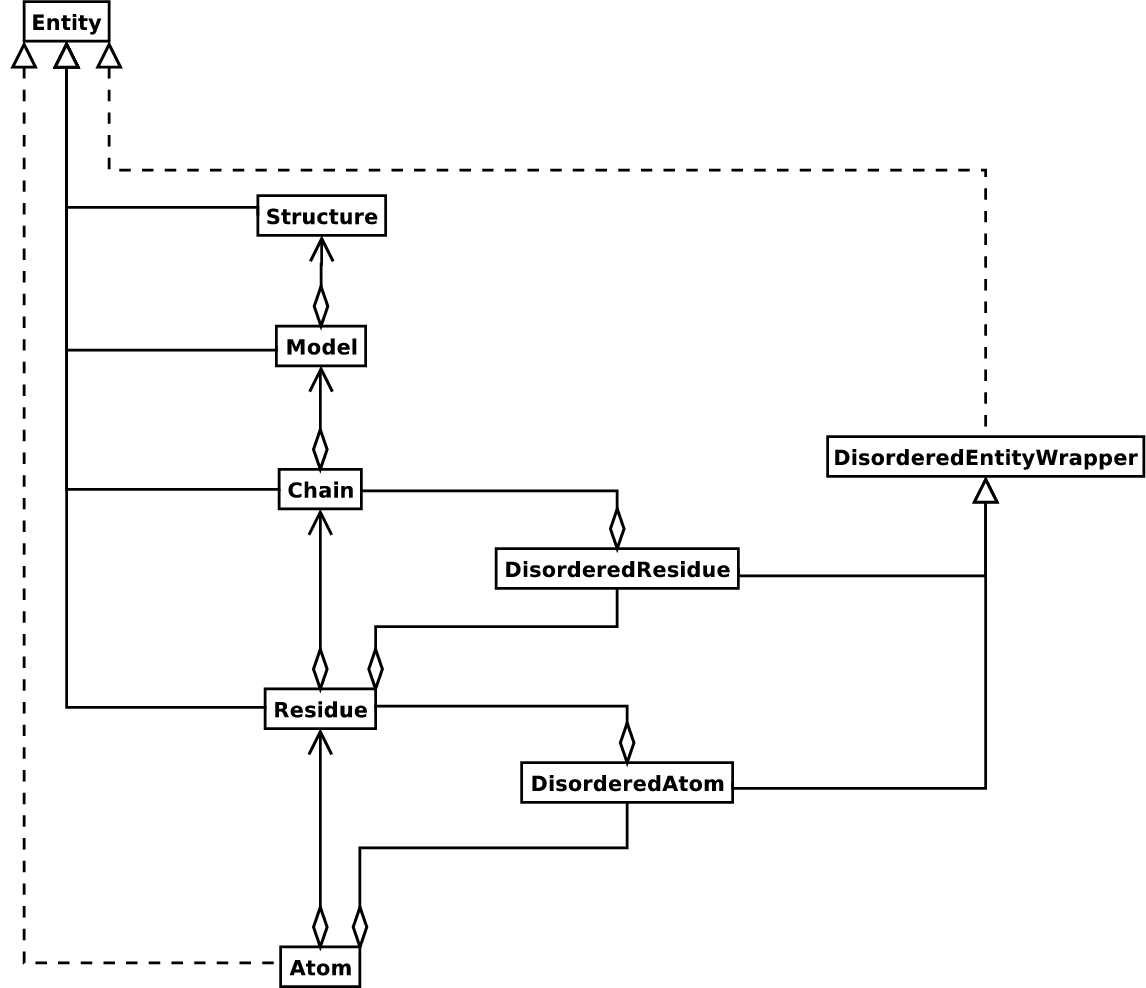
\includegraphics[%
  width=100mm,
  keepaspectratio]{images/smcra.png}\end{center}


\caption{\label{cap:SMCRA}UML diagram of SMCRA architecture of the \texttt{Structure}
object. Full lines with diamonds denote aggregation, full lines with
arrows denote referencing, full lines with triangles denote inheritance
and dashed lines with triangles denote interface realization. }
\end{figure}



\subsubsection*{How do I navigate through a Structure object?}

The following code iterates through all atoms of a structure:

\begin{lyxcode}
p=PDBParser()

structure=p.get\_structure('X',~'pdb1fat.ent')

for~model~in~structure:

~~for~chain~in~model:~

~~~~for~residue~in~chain:

~~~~~~for~atom~in~residue:

~~~~~~~~print~atom
\end{lyxcode}
There are also some shortcuts:

\begin{lyxcode}
\#~Iterate~over~all~atoms~in~a~structure

for~atom~in~structure.get\_atoms():

~~~~print~atom

\#~Iterate~over~all~residues~in~a~model

for~residue~in~model.get\_residues():

~~~~print~residue
\end{lyxcode}
Structures, models, chains, residues and atoms are called \texttt{Entities}
in Biopython. You can always get a parent \texttt{Entity} from a child
\texttt{Entity}, eg.:

\begin{lyxcode}
residue=atom.get\_parent()

chain=residue.get\_parent()
\end{lyxcode}
You can also test wether an \texttt{Entity} has a certain child using
the \texttt{has\_id} method.


\subsubsection*{Can I do that a bit more conveniently?}

You can do things like:

\begin{lyxcode}
atoms=structure.get\_atoms()

residue=structure.get\_residues()

atoms=chain.get\_atoms()
\end{lyxcode}
You can also use the \texttt{Selection.unfold\_entities} function:

\begin{lyxcode}
\#~Get~all~residues~from~a~structure

res\_list=Selection.unfold\_entities(structure,~'R')

\#~Get~all~atoms~from~a~chain

atom\_list=Selection.unfold\_entities(chain,~'A')
\end{lyxcode}
Obviously, \texttt{A=atom, R=residue, C=chain, M=model, S=structure}.
You can use this to go up in the hierarchy, eg.\ to get a list of
(unique) \texttt{Residue} or \texttt{Chain} parents from a list of
\texttt{Atoms}:

\begin{lyxcode}
residue\_list=Selection.unfold\_entities(atom\_list,~'R')

chain\_list=Selection.unfold\_entities(atom\_list,~'C')
\end{lyxcode}
For more info, see the API documentation.


\subsubsection*{How do I extract a specific \texttt{Atom/\-Residue/\-Chain/\-Model}
from a Structure?}

Easy. Here are some examples:

\begin{lyxcode}
model=structure{[}0{]}

chain=model{[}'A'{]}

residue=chain{[}100{]}

atom=residue{[}'CA'{]}
\end{lyxcode}
Note that you can use a shortcut:

\begin{lyxcode}
atom=structure{[}0{]}{[}'A'{]}{[}100{]}{[}'CA'{]}
\end{lyxcode}

\subsubsection*{What is a model id?}

The model id is an integer which denotes the rank of the model in
the PDB/mmCIF file. The model is starts at 0. Crystal structures generally
have only one model (with id 0), while NMR files usually have several
models.


\subsubsection*{What is a chain id?}

The chain id is specified in the PDB/mmCIF file, and is a single character
(typically a letter). 


\subsubsection*{What is a residue id?}

This is a bit more complicated, due to the clumsy PDB format. A residue
id is a tuple with three elements:

\begin{itemize}
\item The \textbf{hetero-flag}: this is \texttt{'H\_'} plus the name of
the hetero-residue (eg. \texttt{'H\_GLC'} in the case of a glucose
molecule), or \texttt{'W'} in the case of a water molecule.
\item The \textbf{sequence identifier} in the chain, eg. 100
\item The \textbf{insertion code}, eg. 'A'. The insertion code is sometimes
used to preserve a certain desirable residue numbering scheme. A Ser
80 insertion mutant (inserted e.g. between a Thr 80 and an Asn 81
residue) could e.g. have sequence identifiers and insertion codes
as follows: Thr 80 A, Ser 80 B, Asn 81. In this way the residue numbering
scheme stays in tune with that of the wild type structure.
\end{itemize}
The id of the above glucose residue would thus be \texttt{('H\_GLC',
100, 'A')}. If the hetero-flag and insertion code are blanc, the sequence
identifier alone can be used:

\begin{lyxcode}
\#~Full~id

residue=chain{[}('~',~100,~'~'){]}

\#~Shortcut~id

residue=chain{[}100{]}
\end{lyxcode}
The reason for the hetero-flag is that many, many PDB files use the
same sequence identifier for an amino acid and a hetero-residue or
a water, which would create obvious problems if the hetero-flag was
not used. 


\subsubsection*{What is an atom id?}

The atom id is simply the atom name (eg. \texttt{'CA'}). In practice,
the atom name is created by stripping all spaces from the atom name
in the PDB file. 

However, in PDB files, a space can be part of an atom name. Often,
calcium atoms are called \texttt{'CA..'} in order to distinguish them
from C$\alpha$ atoms (which are called \texttt{'.CA.'}). In cases
were stripping the spaces would create problems (ie. two atoms called
\texttt{'CA'} in the same residue) the spaces are kept.


\subsubsection*{How is disorder handled?}

This is one of the strong points of Bio.PDB. It can handle both disordered
atoms and point mutations (ie. a Gly and an Ala residue in the same
position). 

Disorder should be dealt with from two points of view: the atom and
the residue points of view. In general, I have tried to encapsulate
all the complexity that arises from disorder. If you just want to
loop over all C$\alpha$ atoms, you do not care that some residues
have a disordered side chain. On the other hand it should also be
possible to represent disorder completely in the data structure. Therefore,
disordered atoms or residues are stored in special objects that behave
as if there is no disorder. This is done by only representing a subset
of the disordered atoms or residues. Which subset is picked (e.g.
which of the two disordered OG side chain atom positions of a Ser
residue is used) can be specified by the user.

\textbf{Disordered atom positions} are represented by ordinary \texttt{Atom}
objects, but all \texttt{Atom} objects that represent the same physical
atom are stored in a \texttt{Disordered\-Atom} object (see Fig. \ref{cap:SMCRA}).
Each \texttt{Atom} object in a \texttt{Disordered\-Atom} object can
be uniquely indexed using its altloc specifier. The \texttt{Disordered\-Atom}
object forwards all uncaught method calls to the selected Atom object,
by default the one that represents the atom with the highest
occupancy. The user can of course change the selected \texttt{Atom}
object, making use of its altloc specifier. In this way atom disorder
is represented correctly without much additional complexity. In other
words, if you are not interested in atom disorder, you will not be
bothered by it.

Each disordered atom has a characteristic altloc identifier. You can
specify that a \texttt{Disordered\-Atom} object should behave like
the \texttt{Atom} object associated with a specific altloc identifier:

\begin{lyxcode}
atom.disordered\_select('A')~\#~select~altloc~A~atom

atom.disordered\_select('B')~\#~select~altloc~B~atom~
\end{lyxcode}
A special case arises when disorder is due to \textbf{point mutations},
i.e. when two or more point mutants of a polypeptide are present in
the crystal. An example of this can be found in PDB structure 1EN2.

Since these residues belong to a different residue type (e.g. let's
say Ser 60 and Cys 60) they should not be stored in a single \texttt{Residue}
object as in the common case. In this case, each residue is represented
by one \texttt{Residue} object, and both \texttt{Residue} objects
are stored in a single \texttt{Disordered\-Residue} object (see Fig.
\ref{cap:SMCRA}).

The \texttt{Dis\-ordered\-Residue} object forwards all un\-caught
methods to the selected \texttt{Residue} object (by default the last
\texttt{Residue} object added), and thus behaves like an ordinary
residue. Each \texttt{Residue} object in a \texttt{Disordered\-Residue}
object can be uniquely identified by its residue name. In the above
example, residue Ser 60 would have id 'SER' in the \texttt{Disordered\-Residue}
object, while residue Cys 60 would have id 'CYS'. The user can select
the active \texttt{Residue} object in a \texttt{Disordered\-Residue}
object via this id.

Example: suppose that a chain has a point mutation at position 10,
consisting of a Ser and a Cys residue. Make sure that residue 10 of
this chain behaves as the Cys residue.

\begin{lyxcode}
residue=chain{[}10{]}

residue.disordered\_select('CYS')
\end{lyxcode}
In addition, you can get a list of all \texttt{Atom} objects (ie.
all \texttt{DisorderedAtom} objects are 'unpacked' to their individual
\texttt{Atom} objects) using the \texttt{get\_unpacked\_list} method
of a \texttt{(Disordered)\-Residue} object.


\subsubsection*{Can I sort residues in a chain somehow?}

Yes, kinda, but I'm waiting for a request for this feature to finish
it :-).


\subsubsection*{How are ligands and solvent handled?}

See 'What is a residue id?'.


\subsubsection*{What about B factors?}

Well, yes! Bio.PDB supports isotropic and anisotropic B factors, and
also deals with standard deviations of anisotropic B factor if present
(see \ref{sub:Analysis}).


\subsubsection*{What about standard deviation of atomic positions?}

Yup, supported. See section \ref{sub:Analysis}.


\subsubsection*{I think the SMCRA data structure is not flexible/\-sexy/\-whatever
enough...}

Sure, sure. Everybody is always coming up with (mostly vaporware or
partly implemented) data structures that handle all possible situations
and are extensible in all thinkable (and unthinkable) ways. The prosaic
truth however is that 99.9\% of people using (and I mean really using!)
crystal structures think in terms of models, chains, residues and
atoms. The philosophy of Bio.PDB is to provide a reasonably fast,
clean, simple, but complete data structure to access structure data.
The proof of the pudding is in the eating.

Moreover, it is quite easy to build more specialised data structures
on top of the \texttt{Structure} class (eg. there's a \texttt{Polypeptide}
class). On the other hand, the \texttt{Structure} object is built
using a Parser/\-Consumer approach (called \texttt{PDBParser/\-MMCIFParser}
and \texttt{Structure\-Builder}, respectively). One can easily re-use
the PDB/mmCIF parsers by implementing a specialised \texttt{Structure\-Builder}
class. It is of course also trivial to add support for new file formats
by writing new parsers.


\subsection{\label{sub:Analysis}Analysis}


\subsubsection*{How do I extract information from an \texttt{Atom} object?}

Using the following methods:

\begin{lyxcode}
a.get\_name()~\#~atom~name~(spaces~stripped,~e.g.~'CA')

a.get\_id()~\#~id~(equals~atom~name)

a.get\_coord()~\#~atomic~coordinates

a.get\_vector()~\#~atomic~coordinates~as~Vector~object

a.get\_bfactor()~\#~isotropic~B~factor

a.get\_occupancy()~\#~occupancy

a.get\_altloc()~\#~alternative~location~specifier

a.get\_sigatm()~\#~std.~dev.~of~atomic~parameters

a.get\_siguij()~\#~std.~dev.~of~anisotropic~B~factor

a.get\_anisou()~\#~anisotropic~B~factor

a.get\_fullname()~\#~atom~name~(with~spaces,~e.g.~'.CA.')
\end{lyxcode}

\subsubsection*{How do I extract information from a \texttt{Residue} object?}

Using the following methods:

\begin{lyxcode}
r.get\_resname()~\#~return~the~residue~name~(eg.~'GLY')

r.is\_disordered()~\#~1~if~the~residue~has~disordered~atoms

r.get\_segid()~\#~return~the~SEGID

r.has\_id(name)~\#~test~if~a~residue~has~a~certain~atom
\end{lyxcode}

\subsubsection*{How do I measure distances?}

That's simple: the minus operator for atoms has been overloaded to
return the distance between two atoms. 

Example:

\begin{lyxcode}
\#~Get~some~atoms

ca1=residue1{[}'CA'{]}

ca2=residue2{[}'CA'{]}

\#~Simply~subtract~the~atoms~to~get~their~distance

distance=ca1-ca2
\end{lyxcode}

\subsubsection*{How do I measure angles?}

This can easily be done via the vector representation of the atomic
coordinates, and the \texttt{calc\_angle} function from the \texttt{Vector}
module:

\begin{lyxcode}
vector1=atom1.get\_vector()

vector2=atom2.get\_vector()

vector3=atom3.get\_vector()

angle=calc\_angle(vector1,~vector2,~vector3)
\end{lyxcode}

\subsubsection*{How do I measure torsion angles?}

Again, this can easily be done via the vector representation of the
atomic coordinates, this time using the \texttt{calc\_dihedral} function
from the \texttt{Vector} module:

\begin{lyxcode}
vector1=atom1.get\_vector()

vector2=atom2.get\_vector()

vector3=atom3.get\_vector()

vector4=atom4.get\_vector()

angle=calc\_dihedral(vector1,~vector2,~vector3,~vector4)
\end{lyxcode}

\subsubsection*{How do I determine atom-atom contacts?}

Use \texttt{NeighborSearch}. This uses a KD tree data structure coded
in C++ behind the screens, so it's pretty darn fast (see \texttt{Bio.KDTree}).


\subsubsection*{How do I extract polypeptides from a \texttt{Structure} object?}

Use \texttt{PolypeptideBuilder}. You can use the resulting \texttt{Polypeptide}
object to get the sequence as a \texttt{Seq} object or to get a list
of C$\alpha$ atoms as well. Polypeptides can be built using a C-N
or a C$\alpha$-C$\alpha$ distance criterion.

Example:

\begin{lyxcode}
\#~Using~C-N~

ppb=PPBuilder()

for~pp~in~ppb.build\_peptides(structure):~

~~~~print~pp.get\_sequence()

\#~Using~CA-CA

ppb=CaPPBuilder()

for~pp~in~ppb.build\_peptides(structure):~

~~~~print~pp.get\_sequence()
\end{lyxcode}
Note that in the above case only model 0 of the structure is considered
by \texttt{PolypeptideBuilder}. However, it is possible to use \texttt{PolypeptideBuilder}
to build \texttt{Polypeptide} objects from \texttt{Model} and \texttt{Chain}
objects as well.


\subsubsection*{How do I get the sequence of a structure?}

The first thing to do is to extract all polypeptides from the structure
(see previous entry). The sequence of each polypeptide can then easily
be obtained from the \texttt{Polypeptide} objects. The sequence is
represented as a Biopython \texttt{Seq} object, and its alphabet is
defined by a \texttt{ProteinAlphabet} object.

Example:

\begin{lyxcode}
>\,{}>\,{}>~seq=polypeptide.get\_sequence()

>\,{}>\,{}>~print~seq

Seq('SNVVE...',~<class~Bio.Alphabet.ProteinAlphabet>)
\end{lyxcode}

\subsubsection*{How do I determine secondary structure?}

For this functionality, you need to install DSSP (and obtain a license
for it - free for academic use, see \url{http://www.cmbi.kun.nl/gv/dssp/}).
Then use the \texttt{DSSP} class, which maps \texttt{Residue} objects
to their secondary structure (and accessible surface area). The DSSP
codes are listed in Table \ref{cap:DSSP-codes}. Note that DSSP (the
program, and thus by consequence the class) cannot handle multiple
models!

%
\begin{table}

\subsubsection*{\begin{tabular}{|c|c|}
\hline 
Code&
Secondary structure\tabularnewline
\hline
\hline 
H&
$\alpha$-helix\tabularnewline
\hline 
B&
Isolated $\beta$-bridge residue\tabularnewline
\hline 
E&
Strand \tabularnewline
\hline 
G&
3-10 helix \tabularnewline
\hline 
I&
$\Pi$-helix \tabularnewline
\hline 
T&
Turn\tabularnewline
\hline 
S&
Bend \tabularnewline
\hline 
-&
Other\tabularnewline
\hline
\end{tabular}}


\caption{\label{cap:DSSP-codes}DSSP codes in Bio.PDB.}
\end{table}



\subsubsection*{How do I calculate the accessible surface area of a residue?}

Use the \texttt{DSSP} class (see also previous entry). But see also
next entry.


\subsubsection*{How do I calculate residue depth?}

Residue depth is the average distance of a residue's atoms from the
solvent accessible surface. It's a fairly new and very powerful parameterization
of solvent accessibility. For this functionality, you need to install
Michel Sanner's MSMS program (\url{http://www.scripps.edu/pub/olson-web/people/sanner/html/msms_home.html}).
Then use the \texttt{ResidueDepth} class. This class behaves as a
dictionary which maps \texttt{Residue} objects to corresponding (residue
depth, C$\alpha$ depth) tuples. The C$\alpha$ depth is the distance
of a residue's C$\alpha$ atom to the solvent accessible surface. 

Example:

\begin{lyxcode}
model=structure{[}0{]}

rd=ResidueDepth(model,~pdb\_file)

residue\_depth,~ca\_depth=rd{[}some\_residue{]}
\end{lyxcode}
You can also get access to the molecular surface itself (via the \texttt{get\_surface}
function), in the form of a Numeric python array with the surface points.


\subsubsection*{How do I calculate Half Sphere Exposure?}

Half Sphere Exposure (HSE) is a new, 2D measure of solvent exposure.
Basically, it counts the number of C$\alpha$ atoms around a residue
in the direction of its side chain, and in the opposite direction
(within a radius of 13 �). Despite its simplicity, it outperforms
many other measures of solvent exposure. An article describing this
novel 2D measure has been submitted.

HSE comes in two flavors: HSE$\alpha$ and HSE$\beta$. The former
only uses the C$\alpha$ atom positions, while the latter uses the
C$\alpha$ and C$\beta$ atom positions. The HSE measure is calculated
by the \texttt{HSExposure} class, which can also calculate the contact
number. The latter class has methods which return dictionaries that
map a \texttt{Residue} object to its corresponding HSE$\alpha$, HSE$\beta$
and contact number values.

Example:

\begin{lyxcode}
model=structure{[}0{]}

hse=HSExposure()

\#~Calculate~HSEalpha

exp\_ca=hse.calc\_hs\_exposure(model,~option='CA3')

\#~Calculate~HSEbeta

exp\_cb=hse.calc\_hs\_exposure(model,~option='CB')

\#~Calculate~classical~coordination~number~exp\_fs=hse.calc\_fs\_exposure(model)

\#~Print~HSEalpha~for~a~residue

print~exp\_ca{[}some\_residue{]}
\end{lyxcode}

\subsubsection*{How do I map the residues of two related structures onto each other?}

First, create an alignment file in FASTA format, then use the \texttt{StructureAlignment}
class. This class can also be used for alignments with more than two
structures.


\subsubsection*{How do I test if a Residue object is an amino acid?}

Use \texttt{is\_aa(residue)}.


\subsubsection*{Can I do vector operations on atomic coordinates?}

\texttt{Atom} objects return a \texttt{Vector} object representation
of the coordinates with the \texttt{get\_vector} method. \texttt{Vector}
implements the full set of 3D vector operations, matrix multiplication
(left and right) and some advanced rotation-related operations as
well. See also next question.


\subsubsection*{How do I put a virtual C$\beta$ on a Gly residue?}

OK, I admit, this example is only present to show off the possibilities
of Bio.PDB's \texttt{Vector} module (though this code is actually
used in the \texttt{HSExposure} module, which contains a novel way
to parametrize residue exposure - publication underway). Suppose that
you would like to find the position of a Gly residue's C$\beta$ atom,
if it had one. How would you do that? Well, rotating the N atom of
the Gly residue along the C$\alpha$-C bond over -120 degrees roughly
puts it in the position of a virtual C$\beta$ atom. Here's how to
do it, making use of the \texttt{rotaxis} method (which can be used
to construct a rotation around a certain axis) of the \texttt{Vector}
module:

\begin{lyxcode}
\#~get~atom~coordinates~as~vectors

n=residue{[}'N'{]}.get\_vector()~

c=residue{[}'C'{]}.get\_vector()~

ca=residue{[}'CA'{]}.get\_vector()

\#~center~at~origin

n=n-ca~

c=c-ca~

\#~find~rotation~matrix~that~rotates~n~

\#~-120~degrees~along~the~ca-c~vector

rot=rotaxis(-pi{*}120.0/180.0,~c)

\#~apply~rotation~to~ca-n~vector

cb\_at\_origin=n.left\_multiply(rot)

\#~put~on~top~of~ca~atom

cb=cb\_at\_origin+ca
\end{lyxcode}
This example shows that it's possible to do some quite nontrivial
vector operations on atomic data, which can be quite useful. In addition
to all the usual vector operations (cross (use \texttt{{*}{*}}), and
dot (use \texttt{{*}}) product, angle, norm, etc.) and the above mentioned
\texttt{rotaxis} function, the \texttt{Vector} module also has methods
to rotate (\texttt{rotmat}) or reflect (\texttt{refmat}) one vector
on top of another.


\subsection{Manipulating the structure}


\subsubsection*{How do I superimpose two structures?}

Surprisingly, this is done using the \texttt{Superimposer} object.
This object calculates the rotation and translation matrix that rotates
two lists of atoms on top of each other in such a way that their RMSD
is minimized. Of course, the two lists need to contain the same amount
of atoms. The \texttt{Superimposer} object can also apply the rotation/translation
to a list of atoms. The rotation and translation are stored as a tuple
in the \texttt{rotran} attribute of the \texttt{Superimposer} object
(note that the rotation is right multiplying!). The RMSD is stored
in the \texttt{rmsd} attribute.

The algorithm used by \texttt{Superimposer} comes from \textit{Matrix
computations, 2nd ed. Golub, G. \& Van Loan (1989)} and makes use
of singular value decomposition (this is implemented in the general
\texttt{Bio.\-SVDSuperimposer} module).

Example:

\begin{lyxcode}
sup=Superimposer()

\#~Specify~the~atom~lists

\#~'fixed'~and~'moving'~are~lists~of~Atom~objects

\#~The~moving~atoms~will~be~put~on~the~fixed~atoms

sup.set\_atoms(fixed,~moving)

\#~Print~rotation/translation/rmsd

print~sup.rotran

print~sup.rms~

\#~Apply~rotation/translation~to~the~moving~atoms

sup.apply(moving)
\end{lyxcode}

\subsubsection*{How do I superimpose two structures based on their active sites?}

Pretty easily. Use the active site atoms to calculate the rotation/translation
matrices (see above), and apply these to the whole molecule.


\subsubsection*{Can I manipulate the atomic coordinates?}

Yes, using the \texttt{transform} method of the \texttt{Atom} object,
or directly using the \texttt{set\_coord} method.


\section{Other Structural Bioinformatics modules}


\subsubsection*{Bio.SCOP}

Info coming soon.


\subsubsection*{Bio.FSSP}

Info coming soon.


\section{You haven't answered my question yet!}

Woah! It's late and I'm tired, and a glass of excellent \textit{Pedro
Ximenez} sherry is waiting for me. Just drop me a mail, and I'll answer
you in the morning (with a bit of luck...).


\section{Contributors}

The main author/maintainer of Bio.PDB is yours truly. Kristian Rother
donated code to interact with the PDB database, and to parse the PDB
header. Indraneel Majumdar sent in some bug reports and assisted in
coding the \texttt{Polypeptide} module. Many thanks to Brad Chapman,
Jeffrey Chang, Andrew Dalke and Iddo Friedberg for suggestions, comments,
help and/or biting criticism :-).


\section{Can I contribute?}

Yes, yes, yes! Just send me an e-mail (thamelry@binf.ku.dk) if you
have something useful to contribute! Eternal fame awaits!


\section{Biopython License Agreement}

Permission to use, copy, modify, and distribute this software and
its documentation with or without modifications and for any purpose
and without fee is hereby granted, provided that any copyright notices
appear in all copies and that both those copyright notices and this
permission notice appear in supporting documentation, and that the
names of the contributors or copyright holders not be used in advertising
or publicity pertaining to distribution of the software without specific
prior permission.

THE CONTRIBUTORS AND COPYRIGHT HOLDERS OF THIS SOFTWARE DISCLAIM ALL
WARRANTIES WITH REGARD TO THIS SOFTWARE, INCLUDING ALL IMPLIED WARRANTIES
OF MERCHANTABILITY AND FITNESS, IN NO EVENT SHALL THE CONTRIBUTORS
OR COPYRIGHT HOLDERS BE LIABLE FOR ANY SPECIAL, INDIRECT OR CONSEQUENTIAL
DAMAGES OR ANY DAMAGES WHATSOEVER RESULTING FROM LOSS OF USE, DATA
OR PROFITS, WHETHER IN AN ACTION OF CONTRACT, NEGLIGENCE OR OTHER
TORTIOUS ACTION, ARISING OUT OF OR IN CONNECTION WITH THE USE OR PERFORMANCE
OF THIS SOFTWARE. 
\end{document}
